\documentclass[12pt]{article}

%Uporabljeni paketi
\usepackage[utf8]{inputenc}
\usepackage{cmap}
\usepackage{type1ec}
\usepackage[T1]{fontenc}
\usepackage{amsthm}
\usepackage{fancyhdr}
\usepackage{graphicx,epsfig}
\usepackage{tabularx,ragged2e,booktabs,caption}
\usepackage{mathtools}
\usepackage[slovene]{babel}
\usepackage{cite}

\usepackage[pdftex,colorlinks,citecolor=black,filecolor=black,linkcolor=black,urlcolor=black,pagebackref]{hyperref}
\usepackage{tikz}

%Velikost strani - dvostransko
\oddsidemargin 1.4cm
\evensidemargin 0.35cm
\textwidth 14cm
\topmargin 0.26cm
\headheight 0.6cm
\headsep 1.5cm
\textheight 20cm

%Nastavitev glave in repa strani
\pagestyle{fancy}
\fancyhead{}
\renewcommand{\sectionmark}[1]{\markright{\textsf{\thesection\  #1}}{}}
%\fancyhead[RE]{\leftmark}
\fancyhead[LO]{\rightmark}
%\fancyhead[LE,RO]{\thepage}
\fancyfoot{}
\renewcommand{\headrulewidth}{0.0pt}
\renewcommand{\footrulewidth}{0.0pt}
\graphicspath{ {images/} }

\newcommand{\gnuplot}{\textbf{gnuplot}}
\newcommand{\pgfname}{\textsc{pgf}}
\newcommand{\tikzname}{Ti\emph{k}Z}
\newtheorem{theorem}{Izrek}
\newtheorem{definicija}{Definicija}
\newtheorem{lema}{Lema}
\begin{document}
\setcounter{page}{1}
\pagenumbering{arabic}

\title{Bitcoin Block Withholding Attack : Analiza in ublažitev napada}
\author{Anej Budihna,Luka Golinar, Matjaz Glumac}


\maketitle
\begin{abstract}

Avtorji se posvetijo dvema problemoma: prvi je študija različice napada imenovanega "bločno prikrivanje" (angl. block withholding attack - BWA) v Bitcoinih in drugi je priporočilo rešitev za preprečitev vseh obstoječih vrst  BWA napadov. Predstavijo analize strategij sebičnega Bitcoin rudarja, ki v potuhi z neko skupino rudarjev poskuša napadati neko drugo skupino in pri tem dobi določeno nagrado, ker je prisostvoval pri napadu na drugo skupino. Tak napad so avtorji poimenovali "sponzorirani napad z bločnim prikrivanjem". Poleg tega predstavijo podrobno kvantitivno analizo dobičkonosnosti, ki jo lahko sebični rudar pridobi s tem, ko rudar uporablja omenjen napad v različnih primerih. V članku avtorji dokažejo, da ob določenih pogojih lahko napadalec optimalno poveča svoj prihodek z uporabo nekaterih strategij in s pametnim izkoriščanjem svojih računalniških virov. Pokažejo tudi, da lahko napadalec uporabi to strategijo za napad na obe skupini, da bi pri tem lahko dosegel višjo dobičkonosnost.
\indent Najpomembneje, predstavijo strategijo, ki se lahko učinkotivto zoperstavi napadu bločnega prikrivanja v katerikoli rudarski skupini. Prvo priporočajo generično shemo, ki uporablja kriptografsko zavezujoče sheme za zoperstavitvi takemu napadu. Nato priporočajo alternativno implementacijo enake sheme z uporabo razpršilnih (angl. hash) funkcij. Taka shema ščiti skupino rudarjev pred zlonamernimi rudarji, tako navadnimi kot tudi administratorskimi redarji. Tako ta shema kot tudi druge njene različice ponujajo obrambo pred BWH napadi s tem, da onemogočijo možnost, da rudarji razlikujejo med celovitimi in delnimi dokazi dela. Prav tako pa te sheme omogočajo zaščito, da administratorji ni omogočeno goljufanje znotraj skupine katero nadzorujejo. Shemo se lahko implementira tako, da se napravi korenito spremembo na obstoječem Bitcoin protokolu.
Na koncu se tudi posvetijo analizi varnosti opisane sheme.

\end{abstract}
{\large \bf Ključne besede:} Bitcoin rudarjenje, napad z bločnim prikrivanjem, sebičen rudar, rudarske skupine, zavezujoče sheme.

\section{Uvod}
Bitcoin je popularna kripto valuta, ki jo je prvo priporočil Satoshi Nakamoto \cite{nakamoto} leta 2008. Transakcije so javno preverljive v glavnem računu imenovanem "bločna veriga" (angl. blockchain). Bločna veriga je sestavljena iz veliko blokov, ki potrdi različne transakcije. Uporabniki, ki ustvarjajo in preverjajo te bloke se imenujejo rudarji. Rudarji nato kot motivacijo pridobijo novo ustvarjene Bitcoin-e. Da bi se reguliralo pretok Bitcoinov se bloki ustvarijo približno vsakih 10 minut. Rudarji morajo rešiti uganko (kot dokaz dela - angl. proof of work (PoW)), če hočejo pridobiti spodbudne Bitcoin-e. Čeprav obstajajo alternativne valute kot Permacoin \cite{permacoin} in Retriecoin \cite{retriecoin}, ki uporabljajo shrambe namesto računanja za ustvarjanje valute, je dokazovanje dela, ki ga uporablja Bitcoin zaenkrat še vedno najboljši načrt. V \cite{economicsofbitcoin} so Kroll  in drugi pokazali, da Bitcoin rudarjenje ni tako "končno", vodeno z vlogami in motivacijsko kompatibilen sistem kot pravijo nekateri njegovi zagovorniki. Napadi z bločnim prikrivanjem \cite{analysisofbitcoin},\cite{financialcryptography}


V \cite{financialcryptography} Laszka in ostali priskrbijo na podlagi igre teoretično analizo napada s prikrivanjem blokov v katerih se pokažejo zanimivi rezultati o dolgolročni vzdržljivosti Nash ravnotežja med napadnjem bazenov v Bitcoin omrežju. Eyal in ostali \cite{minnersdilemma} predlagajo rudarsko igro kjer se bazen rudarjev poskuša vtihotapiti v druge bazne rudarjev tako, da pošlje svoje posamezne rudarje v druge bazene rudarjev kjer potem sprožijo NPB na ciljne bazene rudarjev. Pokazali so, v primeru, da se dva ali več bazenov napada med seboj, bodo pošteni rudarji zaslužili manj kot pričakujejo. V izvornem članku se o takem primeru tudi razpravlja. Vendar se delo avtorjev članka v \cite{originalarticle} razlikuje od dela Eyal in drugih \cite{minnersdilemma} na naslednje načine: (a) Avtorji članka se osredotočijo na znesek dobička, ki ga proizvede napadalec, ki sproži NPB nad nekim ciljnim bazenom rudarjev, katerega nagradi nek drugi bazen rudarjev, ker je napadalec napadel določen bazen rudarjev. Eyal in ostali izračunajo izraze prihodkov, ki jih proizvedejo bazeni rudarjev, ko je scenarij napada omrežja v sanju ravnotežja. (b) V modelu avtorjev \cite{originalarticle} lahko napadalec razdeli svojo računsko moč in tako napada oba bazena rudarjev. Tako lahko prejme nagrade od obeh bazenov, katera nagradita napadalca, ker mislita, da je napadalec napadel le drugi bazen. Toda Eval in drugi razpravljajo scenarij napada kjer so napadalci člani bazena rudarjev in delijo prihodke pridobljene iz napadenega bazena z rudarji v goljufivem bazenu.

\subsection{Motivacija in ostalo delo}

Eyal \cite{minnersdilemma} in ostali definirajo in analizirajo igro kjer identični bazeni rudarjev napadejo drug drugega. Pokazali so, da v takem primeru kjer bazeni rudarjev napadajo drug drugega obstaja Nash ravnotežje, kjer vsi rudarji zaslužijo manj kot če se ne bi napadali drug drugega. Luu in ostali \cite{powersplitting} so izvedli podrobno študijo NPB in pokazali dobiček napadalca ob različnih scenarijih. Dokazali so, da ta napad zares poveča dobiček napadalca. Izpeljali so različne izraze za dobičkonosnost napadalca ob različnih razmerah. Intuicija iza pridobljene napadalčeve spodbude preko NPB je ta, da napadalec uporablja del računske moči za zmanjševanje verjetnosti zmage bazena rudarjev ter tako poveča svoje možnosti za zmago.

V članku \cite{originalarticle} avtorji predlagajo tako imenovani "spozorirani napad s prikrivanjem blokov". Opazili so, da z izvajanjem NPB nad ciljnim bazenom, bo napadalec posredno povečal verjetnost zmage nekateremu drugemu bazenu (kot tudi samemu sebi, če ima dodatne vire za privatno rudarjenje). Zato lahko napadalec kova zaroto z drugimi bazeni, da bo uporabil majhen del svoje moči za napad na nek bazen in posledično zmanjša verjetnosti zmage nad ciljnim bazenom. V takih primerih je lahko napadalec s strani sebičnega bazena za napad na konkurenčni bazen in nagrada naj bi bila proporcionalna glede na narastek spodbude sebičnega bazena, ki ga proizvede napadalec s tem ko napade določen bazen. Tako bo pričakovan narastek napadalca višji kot so to izračunali Luu in ostali v \cite{powersplitting}. To je motivacija za analize avtorjev članka \cite{originalarticle}, ki jo podajo pred koncem razdelka VI v članku \cite{originalarticle}.


NPB lahko ima katastrofalne posledice na dolgoročnost obstanka Bitcoin sistema. V razdelku VI avtorji članka \cite{originalarticle} iščejo oblažitve za NPB. Avtorji članka \cite{originalarticle} predlagajo dejanske ukrepe, ki se lahko uporabijo za premagovanje NPB in tako naredijo Bitcoinove bazene rudarjev bolj varne za investiranje rudarjeve računske moči. Avtorji članka \cite{originalarticle} najprej razpravljajo o generični shemi, ki se jo lahko uporablja poleg kateregakoli kriptografsko zavezujočega protokola. Nato predlagajo različico te sheme, ki uporalja razpršilne funkcije namesto sheme, ki temelji na podlagi zavez. Shema je tako strukturirana, da ne dovoli rudarju, da bi vnaprej predvideval ali lahko kakšen njegov delež uporabljen za generiranje Bitcoinov s strani bazena. Rudar lahko to izve šele nato, ko njen delež v bazenu posredovan k administratorju bazena. O podrobnostih teh shem avtorji članka \cite{originalarticle} razpravljajo kasneje. Opozorilo velja, da naj bi ta protiukrep veljal za vse poznane NPB in ne le za "sponzorirane napade s prikrivanjem blokov".

\subsection{Prispevek}

Prispevek prevedenega članka \cite{originalarticle} je dvonamenski. Članek analizira NPB z mislijo na specifičen model sistema in hkrati predlaga dve rudarski shemi kot oblažitev tem napadom.
\begin{itemize}
	\item V razdelku IV avtorji članka \cite{originalarticle}  analizirajo funkcijo prihodkov napadalca, ki s podporo drugega bazena sproži NPB na ciljni bazen. Ta napad poveča prihodek bazena, ki podpira napadalca in posledično ta bazen lahko del svoje dodatne spodbude z napadalcem. Ta prihodek je glavna opazka na podlagi katere avtorji članka \cite{originalarticle}  izračunajo in analizirajo funkcijo prihodka napadalca. V razdelku V analizirajo dobiček napadalca, ki napade oba bazena.
	Njihova študija je drugačna od \cite{minnersdilemma} v takem smislu, da se študija v  \cite{minnersdilemma} osredotoča na scenarij kjer nek bazen rudarjev pošlje svoje člane, da napade druge bazene. Rudar, ki deluje kot dvojni agent prenese vse svoje pridobljene spodbude nazaj do svojega zlonamernega bazena, kateri nato posreduje dobiček enakomerno med svoje člane. V modelu opisanega v članku \cite{originalarticle} pa rudar deluje neodvisno in dobi neko končno vrednost spodbude od vsakega bloka, ki ga prikrije pred administratorjem bazena.
	\item Glavni rezultati članka so podani v izrekih 1, 2, 3 in 5. Ti rezultati se ukvarjajo z optimalnimi strategijami napadalca pri NPB, ki hoče efektivno uporabiti svoje računske moči, da zasluži kolikor je mogoče. V izreku 1 avtorji članka \cite{originalarticle} dokažejo bistven rezultat, ki ga napadalec lahko uporabi za največji možni dobitek spodbude z oblikovanjem ustrezne strategije napada. 
	V izreku 2 dokažejo da, ko so računske moči bazena vzdrževane na neki konstantni vrednosti, potem napadalec napasti več bazenov istočasno, da se njegov dobiček poveča.
	V izreku 3 pokažejo, da napadalec pridobi več z napadanjem kot s samostojnim rudarjenjem, ko so določeni izvedljivi pogoji izpolnjeni. V izreku 5 pokažejo, da obstaja tak izvedljiv pogoj pod katerim lahko napadalec pridobi največji možni dobiček tako, da napade več bazenov istočasno, ko je računska moč bazenov nekontantna. To pomeni, da napad le na en bazen ne bi pomenilo največjega možnega dobička. Ta ugotovitev je bolj podobna izreku 2. Razlika je ta, da v izreku 5 za razliko od izreka 2, dva bazena nimata vzdrževane računske moči na konstantni vrednosti.
	\item Na koncu, v razdelku VI avtorji predlagajo izboljšavo trenutne Bitcoin sheme na tak način, da bi bilo neobčutljivo na NPB. Prvo predlagajo generično shemo, ki uporablja kriptografsko zavezujoč protokol. Nato predložijo posodobljeno shemo, ki uporablja razpršilno funkcijo namesto zavezujočega protokola. Osnovna ideja za obema shemama je ista. Bolj očitno je, da je druga shema malce preoblikovana prva shema. Avtorji pokažejo, da obe shemi lahko omogočijo odpornost Bitcoin rudarjenja na napade NPB brez ogrožanja ključnih lastnosti obstoječe rudarske sheme. Njihov protiukrep ni samo dober za omenjeni napad v  \cite{originalarticle}, ampak ustreza tudi za vse ostale napade NPB o katerih se razpravlja v \cite{analysisofbitcoin}, \cite{minnersdilemma}, \cite{subversivestrategies}, itd. Dodatki so preprosti za implementacijo in nimajo vpliva na prekomerno računanje dokaza dela.
\end{itemize}

\textit{
	Razdelek VI je neodvisen od razdelkov IV in V brez medsebojnih povezav. Zato lahko bralec, če je zainteresiran samo v spoznavanje obrambnega mehanizma proti NPB, preskoči razdelek VI in V ter nadaljuje neposredno na razdelek VI. }

\subsection{Organizacija}

Preostanek članka  \cite{originalarticle} je organiziran po sledečem vrstnem red: v razdelku II avtorji članka definirajo "dobiček" rudarja in predstavijo bralcu idejo kriptografsko zavezujočega protokola in rudarjenja v Bitcoin sistemu. V razdelku III opišejo model napada in njihove predpostavke v študiji. V razdelku IV avtorji analizirajo spodbudo napadalca, ki napade le posamezen bazen. V razdelku V preučijo spodbudo napadalca, ki napade oba bazena. Na koncu Bag  \cite{originalarticle} in ostali predlagajo izboljšavo na Bitcoin rudarski shemi, s katero se lahko rudarski bazeni obranijo pred NPB. Zaključek članka sledi v razdelku VII.

\section{Predhodna dejanja}
\subsection{Oznake in definicije}
\begin{center}
	
	\begin{tabular} {| c | c | c |}
		\hline
		Serijska št. & Oznaka  & Opis \\ \hline
		1 & $\alpha$ & Računska moč napadalca \\  \hline
		2 & $\beta$ & Delec računske moči, ki je uporabljena za napad na bazen  P \\  \hline
		3 & $\delta$ & Delec  računske moči, ki je uporabljena za napad na bazen P' \\  \hline
		4 & $\gamma$ & Delec dodatnega dobička, ki ga bazen deli z napadalcem \\  \hline
		5 & p & Računska moč bazena P  \\ \hline
		6 & p' & Računska moč bazena P'  \\ \hline
	\end{tabular}
	\captionof{table}{Tabela definicij}
\end{center}

\begin{definicija}
	 Avtorji \cite{originalarticle} uporabljajo isto definijo "dobička" kot v \cite{powersplitting}. Dobiček rudarja je definiran kot delček vrednosti zaslužene spodbude rudarja z rudarjenjem s pomočjo svoje računske moči v skladu s specifično rudarsko strategijo z obzirom do skupno zaslužene spodbude celonega Bitcoin omrežja. $g_m$ predstavlja spodbudo, ki jo zasluži nek določen rudar in $g_B$ pa spodbudo, ki jo zasluži celotno Bitcoin omrežje. Tako potem dobimo dobiček rudarja kot $\frac{g_m}{g_B}$
\end{definicija} 

\subsection{Zavezujoča shema}
Ne-interaktivna zavezujoča shema \cite{datamininglectures} C je sestavljena iz treh verjetnostnih algoritmov polinomnske časovne zahtevnosti \textit{C.Setup()}, \textit{C.Commit()} in \textit{C.Open()}.
\begin{itemize}
	\item \textit{C.Setup($1^k$)} : Ob podanem parametru \textit{k}, bo algoritem \textit{Setup($1^k$)} izpisal javen parameter \textit{CK} zavezujoče sheme.
	\item \textit{C.Commit(CK, x)} : Za parameter x vzame niz $x \in \{0,1\}^k$ in izpiše par  \textit{(com, decom)}. V članku \cite{originalarticle} se zaradi lažjega pisanja včasih izpusti vrednost \textit{decom} in se zapiše  \textit{com} $\leftarrow$ \textit{C.Commit(CK,x)}. Vendar bo bralec zaznal, da ob vsaki izvedbi \textit{C.Commit(CK,x)} bo algoritem izpisal tako zavezujočo kot tudi začetno vrednost.
	\item \textit{C.Open(CK, com, decom)} : Prejme zavezo \textit{com} , prekinitev zaveze \textit{decom} in izpiše x ali simbol za napako $\bot$.
\end{itemize}

\noindent{\large \bfseries Varnostna lastnost }
\newline
\indent Kriptgrafsko zavezujoča shema ima sledeče lastnosti:
\indent Naj bo \textit{C} zavezujoča shema.
\begin{enumerate}
	\item Lastnost skrivanja: Za vse nasprotno verjetnostno polinomske čase \textit{A},
	$|P_r[CK \xleftarrow C.Setup(1^k),(m_0,m_1,st) \leftarrow A(CK), b \xleftarrow{U}  \{0,1\},(com_b, decom_b) \leftarrow C.Commit(CK,m_b) : b = A(CK,st,com_b)] - \frac{1}{2}|  \le negl(k)$
	\item Lastnost vezanja: Za vse nasprotno verjetnostno polinomske čase \textit{A},
	$ Pr[CK \leftarrow C.Setup(1^k),(com,decom,decom') \leftarrow A(CK),m \leftarrow C.Open(com,decom), m' \leftarrow C.Open(com,decom') : m \ne m' \bigwedge m' \ne \bot ] \le negl(k)  $
	\item Sproščeno vezanje: Za vse nasprotno verjetnostno polinomske čase \textit{A},
	$ Pr[CK \leftarrow C.Setup(1^k) , (m,st) \leftarrow A(CK) (com,decom) \leftarrow C.Commit(m,CK), decom' \leftarrow A(CK,st,com,decom'), m \leftarrow C.Open(com,decom') : m \ne m' \bigwedge m' \ne \bot \le negl(k)] $
\end{enumerate}

\section{Sistemski model  za sponzoriran napad s prikrivanjem blokov}

V tem razdelku avtorji članka razpravljajo  o nekaterih predpostavkah, ki so jih uporabili v analizi "sponzoriranih napadov s prikrivanjem blokov" v naslednji dveh razdelkih, v razdelkih IV in V. Bralce opominjamo, da te predpostavke niso povezane z razpravo v razdelku VI, kjer predlagajo proti ukrep proti NPB. V razdelkih IV in V, avtorji upoštevajo model bazena rudarjev z enim samim administratorjem bazena. Odgovornost administratorja je ta ,da koordinira izračune dokaze dela (angl. PoW). Ta izbere množico transakcij in nato določi koren Merkle in ostale parametre. Posamezni rudarji potem poskušajo konstruirati dokaz dela na podlagi teh parametrov. Administrator prav tako nastavi stopnjo zahtevnosti za delne dokaze dela, katere rudarji redno oddajajo administratorju za pregled. Zahtevnostna stopnja delnih dokazov dela je običajno nižja od tiste od Bitcoin sistema, vendar ne sme biti dovolj velika, da preseže kapacitete administratorja. Administrator pregleda vsak delni dokaz dela, ki ga dobi v pregled dokler ne najde enega, ki ustreza zahtevnostni stopnji dokaza o delu (angl. PoW) celotnega Bitcoin omrežja. Če najde kakšen delni dokaz dela, ki ustreza ciljni zahtevnostni stopnji Bitcoin omrežja ga odda Bitcoin sistemu in zahteva nagrado. Avtorji prav tako predpostavijo, da je administrator bazena pošten in da ne more biti skorupiran.

Sedaj sledi podroben opis napada. Bag \cite{originalarticle} in ostali predpostavijo, da je računska moč celonega Bitcoin sistema enaka 1. Imamo dva bazena, P in P'. Naj bo A napadalec čigar računska moč je enaka \textit{a}. Ta razdeli svojo računsko moč na dva dela; prvi del uporablja za samostojno rudarjenje in preostali del uporablja za izvedbo NPB na bazen rudarjev. Napadalec se pridruži ciljnemu bazenu P pod krinko, da je zvest rudar in tako redno oddaja svoje delne dokaze administratorju bazena. Ti deli so le dokazi dela za nizko zahtevnostno stopnjo. Kadarkoli napadalec po naključju najde pravo rešitev, ki ima enako zahtevnostno stopnjo kot celoten Bitcoin sistem, jo prikrije bazenu in je torej ne odda v pregled. Prav tako ne more neposredno oddati te rešitve v celotetn Bitcoin sistem \cite{powersplitting}. Do tega pride, ker obstoječi protokol bazena zahteva, da morajo rudarji oddati block preko administratorja bazena. Tudi če protokol dovoli napadalcu oddajo rešitve neposredno do Bitcoin omrežja, bo začetna transakcija znotraj bloka poskrbela, da bo nagrada odšla neposredno v žep administratorja bazena. Rudar ne bo mogel ohraniti nič dodatnega, razen svojega deleža, ki je enakomerno razdeljen s strani administratorja bazena.

Napadalec namesto tega odda rešitev v bazen P', ki je konkurent bazena P. P' ima skrivnostno zavezo z A. Kadarkoli A prikrije blok bazenu P, ponudi bazen P' nekaj nagrade napadalcu A. P' lahko enostavno preveri pravilnost oddanega bloka s strani napadalca ob predpostavki, da P' pozna množico transakcij na kateri dela bazen P, vključno s transakcijo korena Merkle, kar omogoči P' da preveri dokaz dela, ki ga je napadalec prikril pred bazenom P. Tako lahko predpostavimo, da je bazen P odprt bazen, zato obstaja verjetnost, da bo bazen P' pridobil množico transakcij na kateri dela bazen P. Tako se dobiček napadalca poveča , saj ima sponzorja, ki spodbuja izvajanje napadov na bazen P. Nagrada, ki jo P' da napadalcu $A_1$ je sorazmerna pričakovanemu znesku dobička , ki ga bazen P' proizvede z napadom napadalca A na bazen P. Tako oba, P' in A pridobita na račun računskih virov poštenih rudarjev v bazenu P. Pričakovan dobiček napadalca je višji kot dobiček pri običajnemu NPB , kjer napadalec ne pridobi nobene spodbude s strani konkurenčnih bazenov.

\section{Analiza zaslužene spodbude, ki jo napadalec prejme ob napadu na posamezen bazen}

Avtorji v \cite{powersplitting} so se predvsem osredotočili na študijo dobička napadalca, ki izkorišča NPB za dobiček s strani nekaterega drugega sebičnega bazena. Pomislimo o scenariju kjer imamo dva bazena rudarjev P in P' v celotnem omrežju in enega samega napadalca A. Računska moč napadalca je \textit{a}. Napadalec \textit{A} izkorišča $\beta$ deleža svoje računske moči za rudarjenje v bazenu P in uporablja preostanek $1-\beta$ deleža svoje računske moči za izvajanje samostojnega rudarjenja. Računska moč bazena P in P' so p in p'. Napadalec A rudari v P  z $\alpha \beta $ računske moči in oddaja svoje deleže bazenu le ko deleži ne ustrezajo pravilni rešitvi dejanskega dokaza dela. V primeru da napadalec A dejansko najde veljaven blok, ga le tega ne odda bazenu. Pravtako ga ne more oddati v isti Bitcoin sistem, da bi prejel nagrado. Namesto tega ga odda administratorju bazena P'. Administrator bazena P' da napadalcu nekaj spodbude za izvajanje napada na bazen P in tako poveča verjetnost zmage bazena P'. Razlika med modelom avtorjev članka \cite{originalarticle} in \cite{minnersdilemma} je ta, da v modelu \cite{originalarticle} napadalec izvaja napad neodvisno in ne kot član bazena P'. Zato napadalec ohrani vse morebitne spodbude. V modelu o katerem se govori v \cite{minnersdilemma} deluje napadalec kot zaveznik nekaterega drugega bazena in prenese vse svoje pridobljene spodbude v slabonamerni bazen, kjer se dobiček enakomerno razporedi med člane. Naj bo $\gamma$ delček spodbude, ki jo napadalec prejme od bazena P' za izvajanje NPB na P. Tako predpostavimo, da omrežje nima nobenega drugega igralca, to je

\begin{equation} \label{equation:player}
\alpha(1-\beta) + p + p' = 1 .
\end{equation}

\begin{lema}
	Dobiček, ki ga dobi bazen P', ko napadalec izvede napads prikrivanjem blokov na bazen P, je podan kot  $ G_P$$'= \frac{\alpha \beta p'}{1-\alpha \beta}$.
\end{lema}
\noindent\textit{Dokaz.} Če napadalec uporabi svojo računsko moč, da izvede NPB nad bazenom P, bi bila računska moč celotnega omrežja enaka 1. Tako bi bil pričakovan dobiček za P'  enak p'. Ko pa napadalec uporabi \textit{ $\alpha \beta$} delec svoje računske moči za napad na P, potem pade učinkovita računska moč omrežja na 1 - $\alpha\beta$, zato  dobiček P naraste $\frac{p'}{ 1 - \alpha\beta}$.  Torej je narastek dobička bazena rudarjev P'  $\frac{p'}{1 - \alpha\beta}$ - p' = $\frac{\alpha\beta p'}{1 - \alpha\beta}$




\newpage

\section{Luka - page 5 and forth}


\begin{center}
  \begin{tabular}{ | c | c | c | c | c | }
    \hline
    $\alpha$ & $\beta$ & $\gamma$ & p' & $\bigtriangleup G_h^O $  \\ \hline
    0.200000 & 0.500000 & 0.700000 & 0.340000 & 0.248016 \\ \hline
    0.100000 & 0.900000 & 0.700000 & 0.400000 & 0.417396 \\ \hline
    0.200000 & 0.400000 & 0.700000 & 0.340000 & 0.214171 \\ \hline
    0.160000 & 0.600000 & 0.700000 & 0.330000 & 0.254052 \\ \hline
    0.200000 & 0.800000 & 0.700000 & 0.400000 & 0.394558 \\ \hline
    0.200000 & 0.900000 & 0.700000 & 0.400000 & 0.408747 \\ \hline
    0.200000 & 0.960000 & 0.700000 & 0.400000 & 0.414236 \\ \hline
    0.200000 & 0.990000 & 0.700000 & 0.400000 & 0.416150 \\ \hline
    0.200000 & 0.700000 & 0.700000 & 0.400000 & 0.415573 \\ \hline
  \end{tabular}
\end{center}
TABELA II: Tabelarični prikaz vrednosti $\bigtriangleup G_h^O $ za različne vrednosti ustreznih parametrov. $\alpha$ prikazuje računsko moč napadalca. $\beta$ prikazuje del računske moči, ki jo napadalec uporabi pri napadu na bazen rudarjev P. $\gamma$ prikazuje del spodbude, ki jo bazen P' pridobi zaradi napada napdalaca, ter jo z njim deli. p' predstavlja računsko moč P'.
\newline
\newline

Sedaj je potrebno izračunati spodbudo A. Ker A za napad na P uporablja $\alpha\beta$ del svoje računske moči, lahko predpostavimo, da je računska moč aktivnega omrežja enaka 1 - $\alpha\beta$. Tukaj avtorji predpostavijo\cite{originalarticle}, da so vsi ostali rudarji v baznu P in P' pošteni. Spodbuda A je trojna. Najprej predpostavimo, da je dobiček A zasebnega rudarjenja enaka $ G_1 = \frac{\alpha(1 - \beta)}{ 1 - \alpha\beta}$. Pričakujoč delež spodbude rudarjenja v bazenu P je $ G_2 = \frac{p - \alpha\beta)}{ 1 - \alpha\beta} \frac{\alpha\beta}{p}$. Ponovno je potrebno izpostaviti, da je spodbuda pridobljena iz rudarjenja v bazenu P' zaradi napada na konkurenčni bazen (P) definirana z $ G_3 = G_P' * \gamma = \frac{\alpha\beta p' \gamma}{1 - \alpha\beta} $. 

Torej je skupen dobiček napadalca enaka:
\newline
\begin{equation} \label{eq:2}
G = G_1 + G_2 + G_3 = \frac{\alpha(p-\alpha\beta^2 + p'\beta\gamma)}{p(1 - \alpha\beta)}.
\end{equation}

\textbf{Iz zgornje enačbe so avtorji opazili, da se spodbuda napadalca večka, če napade večji bazen rudarjev, ter dobi spodbudo iz manjšega bazena rudarjev.}
\newline
Avtorji izpostavljajo, da je ko je napadalec uporabil le klasični BWH napad brez tajnega sporazuma z bazenom rudarjev P' je bil pričakovan dobiček enak: $ G = G_1 + G_2 + G_3 = \frac{\alpha(p-\alpha\beta^2 + p'\beta\gamma)}{p(1 - \alpha\beta)}. $ Naraščaj dobičeka, ki ga napadalec pridobi v razmerju z dobičkom originalnega BMH napada se izrazi z:
\newline
\begin{equation} \label{eq:3}
\bigtriangleup G_{BWH}^O = \frac{G}{G'} - 1 = \frac{p'\beta\gamma}{p - \alpha\beta^2}.
\end{equation}

Ker je $ \alpha\beta < p $ je torej $ \alpha\beta^2 < \alpha\beta < p $. Torej avtorji predpostavijo, da je $ \bigtriangleup G_{BWH}^O > 0.$ V primeru, da je bil napadalec pošten rudar je spodbuda, ki jo je precej iz poštenega rudarjenja enaka $G_h = \alpha$. Razmerje spodbude, ki jo napdalec sedaj prejme od tretjih blokov z NPB napadom se izrazi z $\bigtriangleup G_O^h = \frac{G}{G_h} - 1 = \frac{\alpha\beta p + p' \beta\gamma - \alpha\beta^2}{p(1 - \alpha\beta)}$. Če zamenjamo p z $ 1 - p' - \alpha - \alpha\beta$ dobimo,
\begin{equation} \label{eq:4}
\bigtriangleup G_O^h = \frac{G}{G_h} - 1 = \frac{\alpha\beta 1 - p' - \alpha - \alpha\beta + p' \beta\gamma - \alpha\beta^2}{(1 - p' - \alpha - \alpha\beta)(1 - \alpha\beta)}.
\end{equation}
\newline
\begin{figure}
  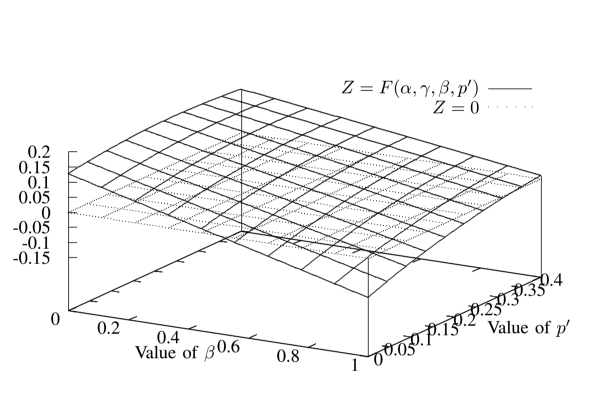
\includegraphics[scale=0.5]{image1.png}
  \caption{Grafični prikaz obnašanja $Z = F(\alpha, \gamma, \beta, p')$, ko sta $\alpha = 0.2, \gamma = 0.7$}
  \label{fig:boat1}
\end{figure}
\newline
\textbf{Izrek 1}. Naj bo $ \beta_0 \in (0, 1) $ tak, da je skupen dobiček napadalca enak $G|_\beta=\beta_0 = max(G|_\beta=\beta_0'): \forall\beta' \in [0,1]$. V tem primeru $\beta_0$ zadosti
\begin{equation}
A \beta_0^2 + B\beta_0 + C = 0
\end{equation}
kjer je $A = -\alpha^2(1 - \gamma)p', B = 4\alpha^2 - 2\alpha^3 - 2\alpha^2p' + 2\alpha p' - 2\alpha, C = \alpha^3 - 2\alpha^2 + 2\alpha^2 p' - 2\alpha p' - \alpha\gamma p' + \alpha + \alpha p'^2 - \gamma p'^2 + \gamma p' $.

\textit{Dokaz.} Dokazali smo, da je v trenutni nastavitvi skupni dobiček napadalca A enak $G = \frac{\alpha(p - \alpha\beta^2 + p'\beta\gamma)}{p(1 - \alpha\beta)}$. V primeru, da p zamenjamo z 1 - p' - $\alpha + \alpha\beta$ v Enačbi(2), dobimo skupni dobiček definiran kot:

\begin{equation}
G = \frac{\alpha(1 - p' - \alpha + \alpha\beta - \alpha\beta^2 + p' \beta\gamma)}{1 - p' - \alpha + \alpha\beta(1 - \alpha\beta)}
\end{equation}

Če diferenciramo po $\beta$, dobimo
$\frac{\partial G}{\partial\beta} = \frac{\alpha(-2\alpha\beta + \gamma p' + \alpha)}{(1 - \alpha\beta)(\alpha\beta - p' - \alpha + 1)} + \frac{\alpha^2(-\alpha\beta^2 + \gamma p'\beta + \alpha\beta - p' - \alpha + 1)}{(1 - \alpha\beta)^2(\alpha\beta - p' - \alpha + 1)} - \frac{\alpha(-\alpha\beta^2 + \gamma p'\beta + \alpha\beta - p' - \alpha + 1)}{(1 - \alpha\beta)(\alpha\beta - p' - \alpha + 1)^2}$. Avtorji so izraz poenostavili, ter dobili $\frac{\partial G}{\partial\beta} = \frac{Num}{Den}$, kjer sta, 
\newline
$Den = (1 - \alpha\beta)^2(1 - p' - \alpha + \alpha\beta)^2$
\newline
$Num = -\alpha^3(1 - \gamma)p'\beta^2 + (4\alpha^3 - 2 \alpha^4 - 2\alpha^3 p' + 2\alpha^2 p' - 2\alpha^2)\beta + (\alpha^4 - 2\alpha^3 + 2\alpha^3 p' - 2\alpha^2 p' - alpha^2\gamma p' + \alpha^2 + \alpha^2 p'^2 - \alpha\gamma p'^2 + \alpha\gamma p')$.
\newline
\newline
Opazimo lahko, da $Den \not= 0 \forall\beta \in [0, 1].$ Če se G razširi nad $\beta = \beta_0, \frac{\partial G}{\partial\beta}|_\beta=\beta_0 = 0$. Torej $-\alpha^3(1-\gamma)p' \beta_0^2 + (4\alpha^3 - 2\alpha^4 - 2\alpha^3 p' + 2\alpha^2 p' - 2\alpha^2)\beta_0 + (\alpha^4 - 2\alpha^3 + 2\alpha^3 p' - 2\alpha^2 p' - \alpha^2 \gamma p' + \alpha^2 + \alpha^2 p'^2 - \alpha\gamma p'^2 + \alpha\gamma p') = 0$. Zaradi tega, ker $\alpha \not= 0$, lahko izraz napišemo kot $-\alpha^2(1 - \gamma)p' \beta^2 + (4\alpha^2 - qalpha\gamma p' + \alpha + \alpha p'^2 - \gamma p'^2 - \gamma p'^2 + \gamma p') = 0$. 
\newline
\newline
\textbf{Lema 2.} Naj bo $ F(\alpha, \gamma, \beta, p') = A\beta^2 + B\beta + C $. V tem primeru je F(.) padajoča funkcija nad $ \beta $, če je $ \alpha $ manjše od 0.25.

Slika 1 prikazuje grafično predstavo vrednosti $ F(\alpha, \gamma, \beta, p') = A\beta^2 + B\beta + C $, kjer so A, B ter C definirani tako kot v Lemi 1. Avtorji so izrisali vrednosti F(.) s tem da so vrednosti $\beta$ in p' variabile, $\alpha$ pa ostaja enak. V primeru, da je p' pod določeno mejo, lahko F(.) zavzame tako negativno, kot pozitivno vrednost. Prav tako lahko opazimo, da F(.) monotono pada, če upoštevamo rezultate Leme 2. Torej lahko sklepamo, obstaja tak $\beta_0$, da je $ F(\alpha, \gamma, \beta, p') = 0 $, kadar je p' pod neko določeno mejo. Podobno, ker je $ F(\alpha, \gamma, \beta, p') > 0 za \beta < \beta_0 $ je G naraščujoča funkcija $\beta$, za $\beta > \beta_0$, kadar je p' majši od omenjene omejitve. Ko je p' najd omenjeno omejitvijo, je G vedno naraščujoča funkcija. Za napadalca se v tem primeru najbolj splača inverstirati vse svoje računske zmožnosti v bazen rudarjev P. V primeru ko je vrednost p' dovolj nizka, obstaja tak $\beta \in [0, 1]$, ki omogoča maksimalen dobiček. Ta $\beta_0$ ustreza križišču dveh krivulj $Z = F(\alpha, \gamma, \beta, p')$ in Z = 0 na Sliki 1. Vrednost $\beta_0$ lahko dobimo tako, da rešimo kvadratično enačbo $A\beta^2 + B\beta + C = 0$. Vrednost $\beta_0$, ki najbolj poveča dobiček napadalca je $\{\frac{-B - 4AC}{2A}, \frac{-B -4AC}{2A}\}$.
\newline
Potrebno je izpostaviti, da v primeru, da F(.) monotono pada, obstaja natanko ena vrednost $\beta_0$, ki maksimizira dobiček G. Zaradi tega veljata $0 < \frac{-B-4AC}{2A} < 1$ ali pa $0 < \frac{-B - 4 AC}{2A} < 1$, nikakor pa ne oba hkrati.

\subsection{NAPAD NA OBA BAZENA RUDARJENJA HKRATI}
Ponovno si predstavljamo situacijo, v kateri napadalec napade hkrati bazen rudarjev P ter P'. Tako prej, lahko predpostavljamo, da je napadalčeva računska moč enaka $\alpha$. Napadalec razdeli računsko moč na tri dele; $A_1, A_2, A_3$, z računsko močjo enako $\alpha\beta$, $\alpha\delta$ in $1 - \alpha\beta - \alpha\delta$. Napadalec uporabi $\alpha\beta$ njegove računske moči za napad P ter pridobitev spodbude P'. Podobno, uporabi $\alpha\delta$ njegove procesorske moči in tako napade P' ter pridobi spodbudo od P. Na ta način, bo pričakavoma spodbuda napdalčevega osebnega rudarjenja enaka $ G = \frac{\alpha(1 - \beta - \delta)}{1 - \alpha\delta - \delta\gamma}$. Delež nagrade, ki ga pridobi iz P je izražen kot $G_2 = \frac{p - \alpha\beta}{1 - \alpha(\beta + \delta)} \frac{\alpha\beta}{p}$. Nagrada pridobljena z rudarjenjem bazena P' se poda z $G_3 = \frac{p' - \alpha\delta}{1 - \alpha\beta - \alpha\delta} \frac{\alpha\delta}{p'}$. Spodbuda, ki jo napadalec dobi zaradi napada na P pa je podana z $G_4 = \frac{\alpha\beta p' \gamma}{1 - \alpha\beta}$. Podobno je definirana tudi spodbuda, ki jo napadelc pridobi z bazena P, zaradi napada na P'; $G_5 = \frac{\alpha\delta p \gamma}{1 - \alpha\delta}$. Predpostavimo lahko torej, da je skupni dobiček napadalca predstavljen kot $G = \Sigma_{i=1}^5 G_i = \frac{\alpha - \alpha\beta - \alpha\delta}{1 - \alpha\beta - \alpha\delta} + \frac{p \alpha\beta - \alpha^2\beta^2}{p(1 - \alpha\beta - \alpha\delta)} + \frac{p' \alpha\delta - \alpha^2\delta^2}{p'(1 - \alpha\beta - \alpha\delta)} + \frac{\alpha\beta p' \gamma}{1 - \alpha\beta} + \frac{\alpha\delta p \gamma}{1 - \alpha\delta}$
\newline
\newline
\textit{A. Ko so računske moči rudarskih bazenov konstantne}
V nasledjem primeru si bomo ogledali spodbudo napadalca, ki napada bazen P in P' hkrati. Najprej predpostavimo, da sta računski moči P in P' konstatni čez celotno periodo. To se zgodi, ko rudar vloži v bilo kateri bazen vlogi nekaj dodatne procesorske moči, administrator bazena izključi nekaj svojih sistemov, ter na ta način vzdržuje konstantno procesorsko moč. Drugi način pa se zgodi, ko nekaj rudarjev zapusti bazen. Takrat sistemski administrator vključi nekaj svojih resursov in tako nadoknadi izgubo. Na ta način zagotovimo konstantko računsko moč P in P'. Na ta način obržimo režijske stroške administratorju bazena konstantne. Tako, kot smo to opisali prej, člani bazena administratorju konstantno delne dokaze njihovega dela. Administrator bazena lahko tako preveri, da vsi njegovi člani v bazen res vlagajo dogovorjeno računsko moč. Vsako odstopanje, se izraža v številu in frekvenci oddanih vložkov. To povzroči dodatne režiske stroške na administratorja bazena. Zaradi tega razloga, se administrator trudi obdržati režiske stroške konstantne. Torej, se napadalec trudi obdržati odstopanja rudarske moči zaradi izstopa enega ali dve rudarjev čim manjšo. Lahko bi diskutirali razmišljanje za tako hipotezo, saj v večini primerov, rudarski bazeni nimajo nikoli konstane moči računanja zgoščevalne funkcije. Avtorji povdarjajo, da se konstantna procesroska moč predpostavi zaradi lažjega analize in ne za prikaz realističnega primera. V sekciji V-B smo analizirali scenarij, kjer se računska moč bazena zaradi izhoda in prihoda novih rudarjev spreminja. Bralec lahko ta razdelek smatra kot vstopna točka za razdelek V-B.

\textbf{Izrek 2}. Naj bo A napadalec, ki uporabla frakcijo e njegove procesorske moči pri napadu na bazen P in P'. Primer: $\beta + \delta = e$. Obstaja tudi taka enolična vrednost $\beta_0 \in (0, e)$, da je napadalčev dobiček G maksimiziran za $\beta = \beta_0$, če velja naslednji pogoj:
\begin{equation}
\gamma p'^2 + \frac{2\alpha e}{1 - \alpha e > \frac{\gamma p p'}{(1 - \alpha e)^2}}.
\end{equation}

\textit{Dokaz}. Skupni dobiček napadalca $G = \frac{\alpha - \alpha\beta - \alpha\delta}{1 - \alpha\beta - \alpha\delta} + \frac{p \alpha\beta - \alpha^2\beta^2}{p(1 - \alpha\beta - \alpha\delta)} + \frac{p'\alpha\delta - \alpha^2\delta^2}{p'(1 - \alpha\beta - \alpha\delta)} + \frac{\alpha\beta p' \gamma}{1 - \alpha\beta} + \frac{\alpha\delta p \gamma}{1 - \alpha\delta}$. Zamenjamo $\delta$ z e - $\alpha$ in dobimo $G = \frac{\alpha(1 - e)}{1 - \alpha e} + \frac{p \alpha\beta - \alpha^2\beta^2}{p(1 - \alpha e)} + \frac{p' \alpha(e - \beta) - \alpha^2(e - \beta)^2}{p'(1 - \alpha e)} + \frac{\alpha(\beta p' \gamma)}{1 - \alpha\beta} + \frac{\alpha(e - \beta) p \gamma}{1 - \alpha(e - \beta}$. Uporabimo delni odvod in dobimo: $\beta, \frac{\partial G}{\partial \beta} = \frac{p\alpha - 2\alpha^2\beta}{p(1 - \alpha e)} + \frac{-p' \alpha + 2 \alpha^2(e - \beta)}{p' (1- \alpha e)} + \frac{\alpha\gamma p'}{(1 - \alpha\beta)^2} - \frac{\alpha\gamma p'}{(1 - \alpha\beta)^2} - \frac{\alpha\gamma p}{(1 - \alpha(e - \beta)) ^ 2}$

\begin{equation}
\frac{\partial G}{\partial \beta} |_{\beta=0} = \frac{2\alpha^2 e}{p' (1 - \alpha e)} + \alpha\gamma p' - \frac{\alpha\gamma p }{(1 - \alpha e)^2}.
\end{equation}
\begin{equation}
\frac{\partial G}{\partial \beta} |_{\beta=e} = -\frac{2\alpha^2 e}{p' (1 - \alpha e)}- \frac{\alpha\gamma p' }{(1 - \alpha e)^2} + \alpha\gamma p.
\end{equation}
Ker je $\gamma p'^2 + \frac{2\alpha e}{1 - \alpha e} - \frac{\gamma}{(1 - \alpha e) ^ 2} p p' > 0$
\begin{equation}
\alpha\gamma p' + \frac{2\alpha^2 e}{p'(1 - \alpha e)} - \frac{\alpha\gamma p}{(1 - \alpha e)^2} > 0.
\end{equation}
Zaradi tega, ker je P večji bazen je p > p'. Torej je $\gamma p^2 + \frac{2\alpha e}{1 - \alpha e} - \frac{\gamma}{(1 - \alpha e)^2} p p' > 0$. Torej,
\begin{equation}
\alpha\gamma p + \frac{2\alpha^2 e}{p(1 - \alpha e)} - \frac{\alpha\gamma p'}{(1- \alpha e)^2} > 0.
\end{equation}

\newpage 
Stran 9 naprej

Potem v razdelku VI-B je prikazano kako lahko isto shemo implementiramo z uporabi razpršitvenih funkcij, ki je v nekem smislu sama po sebi zavezujoča shema. Vseeno pa je potrebno opraviti majhen popravek na izvorni shemi, da to lahko deluje. Shema avtorjev v \cite{originalarticle} se brani pred NPB tako, da onemogoča rudarjem možnost, da bi bili sposobni razlikovati med delnim dokazom dela in med celovitim dokazom dela.

\subsection{Shema 1}

V obstoječi Bitcoin shemi mora rudar izračunati \textit{"nonce" n} (nonce je 32 bitno polje v Bitcoin bloku)  in Bitcoin blok ki vsebuje "nonce" in transakcije tako, da bo razpršilna vrednost v glavi bloka vsebovala \textit{z} vodilnih '0' bitov. Temu rečemo "tarča" dokaza dela. Torej bo tarča niz bitov z dolžino \textit{z}. V trenutnem Bitcoin rudarskem protokolu je tarča niz, ki ima \textit{z} število bitov z vrednostjo 0. Tako je pravilno zgrajen Bitcoin blok čigar razpšilna vrednost z razpršilno funkcijo SHA-256 vrne niz ,ki se začne z \textit{z} številom bitov z vrednostjo 0, zmagoviti blok, ki lahko dobrinese dobiček v višini 25BTC iz Bitcoin sistema. Delni dokazi dela, ki se neprestano oddajajo v pregled dela  administratorju bazena  s strani rudarjev v bazenu, imajo ciljni bitni niz čigar velikost je \textit{z} kjer je {$ z' \le z $}. Vrednost z' določi administrator bazena in mora biti taka, da lahko rudarji v bazenu konstantno poiščejo delne dokaze dela, vendar preverjanje teh delnih dokazov ne sme predstavljati prevelikega računskega bremena administratorju bazena. Tako so avtorji \cite{originalarticle} dopolnijo trenutno shemo in predlagajo novo, v kateri bazen lahko sam izbera tarčo. Predlagana shema deluje po naslednjih korakih:
\begin{itemize}
	\item V shemi avtorjev se kot v obstoječi shemi pusti administratorju bazena odločitev koliko bitnih vrednosti "0" je potrebnih v delnih dokazih dela, da jih lahko posamezni rudarji oddajo administratorju. Naj bo \textit{z'} kjer je \textit{$z' \le z$}. Delni dokaz dela je blok čigar razpršitvena vrednost se začne s številom \textit{z'} ničelnih bitov.
	\item Bazen rudarjev izbere \textit{$z - z'$} najmanj pombembnih bitov ciljnega celovitega dokaza dela. Naj bo to \textit{r}, $r \in \{0, 1\} z - z'$ . Bazen izbere tudi naključen niz $s \in \{0, 1\}^*$ , kjer je \textit{$ |s| + |r| = k$}, kjer je \textit{k} varnostni parameter zavezujoče sheme, ki jo definira Bitcoin sistem in ne bazen sam. Tukaj je vloga \textit{s} ta, da naredi dolžino združenega "nonce" \textit{$r||s$} enako \textit{k}, ki je predpisana dolžina zavezujoče sheme. Vrednost varnostnega parametra naj bi bila taka, da naj bi bil "zlom" zavezujoče sheme težji kot iskanje celovitega dokaza dela. Splošno lahko uporabimo kot varnostni parameter 256 za shemo avtorjev \cite{originalarticle}. Glavna razlika med shemo avtorjev in trenutno rudarsko shemo je ta, da v shemi avtorji bazen določi zadnjih \textit{$ z - z' $} zadnjih bitov tarče, ki je lahko v obliki $\{0, 1\}^{z-z'}$.
	\item Končna tarča celovitega dokaza dela bazena tako postane \textit{$0^{z'}||r$}, ki je dolžine \textit{z} in je enake dolžine kot tarča trenutne Bitcoin rudarske sheme.
	\item Bazen rudarjev proizvede zavezo \textit{$(com, decom) \leftarrow - Commit(r||s, CK)$}. Bazen pošlje zavezo vsem rudarjem in zaenkrat ohrani začetno vrednost \textit{decom} skrito.
	\item  Vsi rudarji bazena vključijo zavezo \textit{com} in \textit{z'} v dokazih dela, ki ga izračunajo. Ko rudar zgradi blok se zaveza \textit{com} in dolžina tarče delnega dokaza prav tako vključi v blok. Delni dokazi vkjučujejo vse bloke katerih razpršitvena vrednost se začne z $0^{z'}$. Tako lahko rudar odda vse bloke, ki imajo razpršitvene vrednosti enake $0^{z'}||\{0, 1\}^*$
	\item Administrator bazena prejme kot delne dokaze vse bloke katerih razpršitvena vrednost se začne z $0^{z'}$. Sedaj administrator pregleduje te delne dokaze dokler ne najde celovitega dokaza, ki vsebuje razpršitveno vrednost, ki se začne z $0^{z'}||r$. Če lahko najde takšen blok, potem odda ta blok v Bitcoin sistem skupaj z začetno zavezo \textit{decom}. 
	\item Ko vozlišča Bitcoin omrežja prejmejo ta blok in začetno vrednost \textit{decom} bodo izluščili vrednost zaveze \textit{com} in \textit{z'}, ki sta vsebovani v bloku in nato izluščijo \textit{$ r||s \leftarrow Open(com,decom)$}. Blok je sprejet, če se izkaže da je prvih \textit{z} bitov razpršitvene vrednosti enakih $0^{z'}||r$, kjer je \textit{r} prvih \textit{$z-z'$} bitov iz \textit{Open(com, decom)}. Če je kaj neskladja, se blok zavrne. Opozoriti velja, da je lahko vrednost \textit{z'} med bazeni različna. Vseeno lahko Bitcoin vozlišče poišče isto vrednost za določen bazen v oddanem bloku bazena. Če se razpršitvena vrednost bloka začne z \textit{'1'}, potem mora biti vrednost \textit{z} za blok enaka 0.
\end{itemize}

\noindent\textbf{Varnostna lastnost predlagane sheme:} Tukaj avtorji \cite{originalarticle} pokažejo, da je njihova shema varna pred NPB. Pokažejo tudi, da ta shema ne omogoča nobenega maneverskega prostora kateremukoli bazenu rudarjev za reševanje rudarske uganke z uporabo manjše količine računske moči kakršno sami pričakujejo. To pomeni, da shema ne omogoča lažje poti do zmage pri rudarski igri. Trdnost predlagane sheme je enaka kot pri obstoječi Bitcoin shemi in rudarji ne dobijo nobene prednosti v primerjavi z obstoječo shemo.

Enostavno je videti, da je predlagana shema odporna na NPB, ki jo izvedejo rudarji, saj rudarji vedo le "tarčo" delnega dokaza dela ($O^{z'}$) in jim ni dovoljeno, da bi vedeli ostalih $z-z'$ bitov \textit{(r)} iz katerega je sestavlen celovit dokaz dela, dokler ni rudarsko delo osveženo, zaradi pojavitve Bitcoin bloka, ki ga je zgradil nek drugi bazen, ki vsebuje eno ali več transakcij iz množice transakcij nad katerimi rudarijo rudarji iz trenutnega bazena. Rudarji izvedo le zavezo \textit{com} k kombiniranemu "nonce" \textit{r||s} in prvih nekaj bitom (\textit{r}) ne morejo poznati iz zaveze \textit{com} zaradi lastnosti skrivanja, ki jo ima zavezujoča shema. Tako rudarji ne morejo razlikovati med delnim dokazom dela in celovitim dokazom dela. Zaradi tega ne morejo prikriti veljavne rešitve. Avtorji dokažejo varnost sheme v  Lemi \ref{lema3} in 4.

\begin{lema}\label{lema3}
	Predlagano rudarjenje zagotavlja, da bazen rudarjev ne more ugotoviti dokaz dela z uporabo manj računske moči kot bi jo morali.
\end{lema}

\noindent \textit{Dokaz.} Če bazen rudarjev poskuša pretentati obstoječo rudarsko shemo, mora storiti naslednje; Predpostavimo, da bazen rudarjev izbere dvobitna niza \textit{r} in \textit{s} tako, da je \textit{$|r| + |s| = K$} in potem izračuna zavezo \textit{$com \leftarrow Commit(r||s, CK)$}.

\newpage
\begin{thebibliography}{9}
 
 \bibitem{nakamoto}
 S. Nakamoto, 
 \textit{Bitcoin: A peer-to-peer electronic cash system}, 2008.
 
 \bibitem{permacoin}
 A. Miller, A. Juels, E. Shi, B. Parno, and J. Katz, 
 \textit{Permacoin: Repurposing bitcoin work for data preservation}, in 2014 IEEE Symposium on Security and Privacy, SP 2014, Berkeley, CA, USA, May 18-21, 2014. IEEE Computer Society, 2014, pp. 475–490.
 
 \bibitem{retriecoin}
 B. Sengupta, S. Bag, S. Ruj, and K. Sakurai, 
 \textit{Retricoin: Bitcoin based on compact proofs of retrievability}, in Proceedings of the 17th International Conference on Distributed Computing and Net- working, ser. ICDCN ’16, 2016, pp. 14:1–14:10.
 
 \bibitem{economicsofbitcoin}
 J. A. Kroll, I. C. Davey, and E. W. Felten, 
 \textit{The economics of bitcoin mining, or bitcoin in the presence of adversaries,}Proceedings of WEIS, vol. 2013, 2013.
 
 \bibitem{analysisofbitcoin}
 M. Rosenfeld,
 \textit{Analysis of bitcoin pooled mining reward systems}, CoRR, vol. abs/1112.4980, 2011. [Online]. Available: http://arxiv.org/abs/1112.4980
 
 \bibitem{financialcryptography}
 A. Laszka, B. Johnson, and J. Grossklags, 
 \textit{Financial Cryptography and Data Security: FC 2015 International Workshops, BITCOIN, WAHC, and Wearable, San Juan, Puerto Rico, January 30, 2015, Revised Selected Papers.} Berlin, Heidelberg: Springer Berlin Heidelberg, 2015, ch. When Bitcoin Mining Pools Run Dry, pp. 63–77.
 
 \bibitem{minnersdilemma}
 . Eyal, 
 \textit{The miner’s dilemma}, in 2015 IEEE Symposium on Security and Privacy, SP 2015, San Jose, CA, USA, May 17-21, 2015. IEEE Computer Society, 2015, pp. 89–103.
 
 \bibitem{powersplitting}
 L. Luu, R. Saha, I. Parameshwaran, P. Saxena, and A. Hobor, 
 \textit{On power splitting games in distributed computation: The case of bit- coin pooled mining}, in IEEE 28th Computer Security Foundations Symposium, CSF 2015, Verona, Italy, 13-17 July, 2015, C. Fournet, M. W. Hicks, and L. Vigano`, Eds. IEEE Computer Society, 2015, pp. 397–411.
 
 \bibitem{subversivestrategies}
 N. T. Courtois and L. Bahack, 
 \textit{On subversive miner strategies and block withholding attack in bitcoin digital currency}, arXiv preprint arXiv:1402.1718, 2014.
 
 \bibitem{datamininglectures}
 I. Damg{\'a}rd, 
 \textit{Lectures on Data Security: Modern Cryptology in The- ory and Practice.} Berlin, Heidelberg: Springer Berlin Heidelberg, 1999, ch. Commitment Schemes and Zero-Knowledge Protocols, pp. 63–86.
 
 \bibitem{incentivecompability}
 D. B. Okke Schrijvers, Joseph Bonneau and T. Roughgarde, 
 \textit{In- centive compatibility of bitcoin mining pool reward functions}, in Financial Cryptography and Data Security: FC 2016 International Workshops.
 
 \bibitem{noteonblockattack}
 S. Bag and K. Sakurai, 
 \textit{Yet another note on block withholding attack on bitcoin mining pools}, in Information Security - 19th International Conference, ISC 2016, Honolulu, HI, USA, September 3-6, 2016, Proceedings, ser. Lecture Notes in Computer Science,
 M. Bishop and A. C. A. Nascimento, Eds., vol. 9866. 2016, pp. 167–180.
 
 \bibitem{originalarticle}
 Samiran Bag, Sushmita Ruj and Kouichi Sakurai,
\textit{Bitcoin Block Withholding Attack : Analysis and
Mitigation}
IEEE Transactions on Information Forensics and Security
\end{thebibliography}
\end{document}

